\documentclass[aspectratio=169]{beamer}
\usetheme[faculty=phil]{fibeamer}
\usepackage{polyglossia}
\setmainlanguage{english} %% main locale instead of `english`, you
%% can typeset the presentation in either Czech or Slovak,
%% respectively.
\setotherlanguages{russian} %% The additional keys allow
%%
%%   \begin{otherlanguage}{czech}   ... \end{otherlanguage}
%%   \begin{otherlanguage}{slovak}  ... \end{otherlanguage}
%%
%% These macros specify information about the presentation
\title[AGLA2]{Analytical Geometry and Linear Algebra II, Lab 3} %% that will be typeset on the
\subtitle{Null space \\ \ \\ \ 
         } %% title page.
\author{Oleg Bulichev}
%% These additional packages are used within the document:
\usepackage{ragged2e}  % `\justifying` text
\usepackage{booktabs}  % Tables
\usepackage{tabularx}
\usepackage{tikz}      % Diagrams
\usetikzlibrary{calc, shapes, backgrounds}
\usepackage{amsmath, amssymb}
\usepackage{url}       % `\url`s
\usepackage{listings}  % Code listings
% \usepackage{subfigure}
\usepackage{floatrow}
\usepackage{subcaption}
\usepackage{mathtools}
\usepackage{todonotes}
\usepackage{fontspec}
\usepackage{multicol}
\graphicspath{{resources/}}
\frenchspacing

\setbeamertemplate{caption}[numbered]
\usetikzlibrary{graphs}

% \usepackage[backend=biber,style=ieee,autocite=footnote]{biblatex}
% \addbibresource{biblio.bib}
% \DefineBibliographyStrings{english}{%
%   bibliography = {References},}

\newcommand{\oleg}[2][] {\todo[color=red, #1] {OLEG:\\ #2}}
\newcommand{\fbckg}[1]{\usebackgroundtemplate{\includegraphics[width=\paperwidth]{#1}}}%frame background

\usepackage[framemethod=TikZ]{mdframed}
\newcommand{\dbox}[1]{
\begin{mdframed}[roundcorner=3pt, backgroundcolor=yellow, linewidth=0]
\vspace{1mm}
{#1}
\vspace{1mm}
\end{mdframed}
}

\begin{document}
\fbckg{fibeamer/figs/title_page.png}
\frame[c]{\setcounter{framenumber}{0}
    \usebeamerfont{title}%
    \usebeamercolor[fg]{title}%
    \begin{minipage}[b][6.5\baselineskip][b]{\textwidth}%
        \textcolor{black}{\raggedright\inserttitle}
    \end{minipage}
    % \vskip-1.5\baselineskip

    \usebeamerfont{subtitle}%
    \usebeamercolor[fg]{framesubtitle}%
    \begin{minipage}[b][3\baselineskip][b]{\textwidth}
        \raggedright%
        \insertsubtitle%
    \end{minipage}
    \vskip.25\baselineskip
}
%   \frame[c]{\maketitle}

\fbckg{fibeamer/figs/common.png}


% \section{Introduction}
% \begin{frame}[t]{\insertsectionhead}


\begin{frame}[t]{How to study Null Space}
    \framesubtitle{Step-by-step guide}
    \vspace{-0.65cm}
    \small
    \begin{enumerate}
        \item \href{https://youtu.be/8o5Cmfpeo6g}{Lecture 6, Gilbert Strang} \\ \textbf{Goal} is to understand the basics of spaces and how Null Space appeared.
        \item \href{https://www.youtube.com/watch?v=_uTAdf_AsfQ}{Khan Academy: Null space} \\ It contains a good case study how to calculate Null space.
        \item \href{https://www.youtube.com/watch?v=C8zOd07U3l8}{Matrix Algebra for Engineers: Null Space} \\ Another nice example how to find $N(A)$.
        \item \textit{"Linear Algebra and Applications", pdf pages 96--106 } \\ What does partial and full solutions means
        \item \href{https://www.youtube.com/watch?v=ggWYkes-n6E}{The Big Picture of Linear Algebra} \\ \textit{Extra for now} If you want to get the global view of four subspaces
        \item Understand the application from next few slides and make HW tasks!
    \end{enumerate}
\end{frame}

\begin{frame}[t]{Null Space: Application from robotics}
    \framesubtitle{Video}
    \vspace{-0.6cm}
    \begin{figure}[H]
        \href{https://youtu.be/sZYBC8Lrmdo}{
            \centering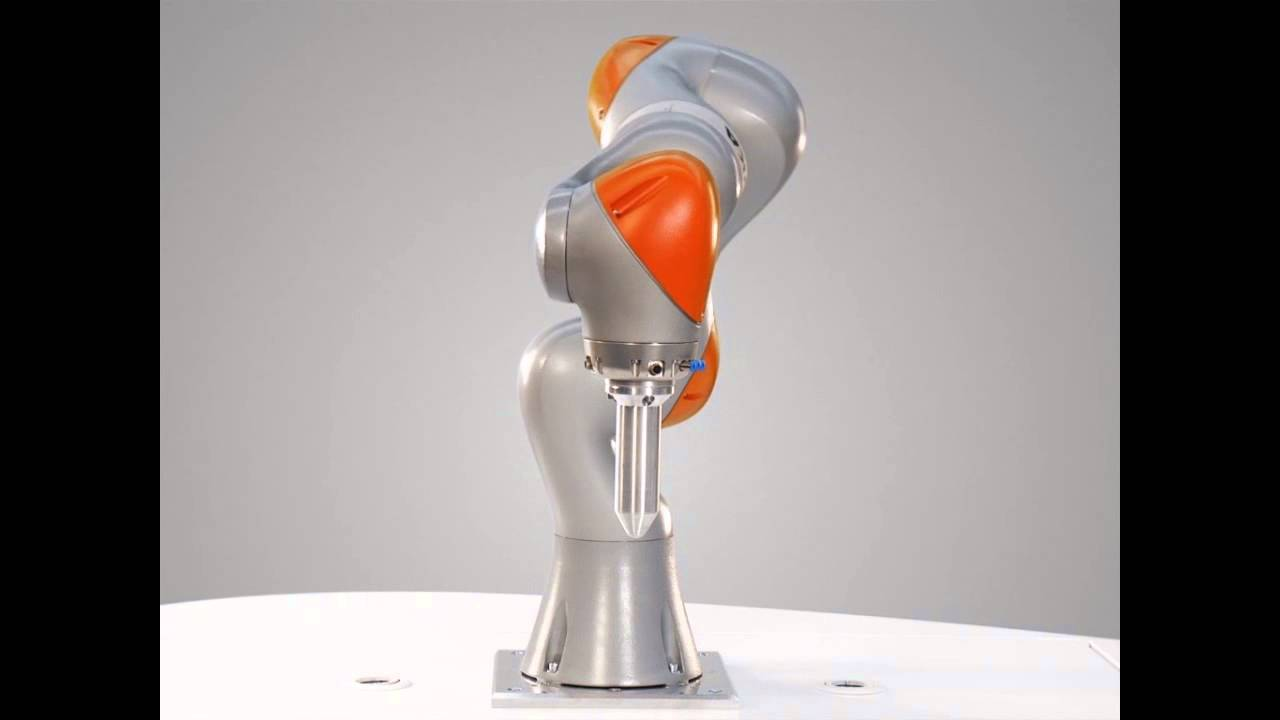
\includegraphics[height=6cm,width=1\textwidth,keepaspectratio]{kuka.jpg}}
        % \caption{Click on a picture for a video}
        \label{fig:kuka.jpg}
    \end{figure}
\end{frame}

\begin{frame}[t]{Null Space: Application from robotics}
\framesubtitle{Theory (1)}
\begin{columns}[T,onlytextwidth]
\begin{column}{0.46\textwidth}
\begin{figure}[H]
    \href{https://colab.research.google.com/drive/1VJGLiDYiWY2EeecCETGjEkZpjaqL8v5e?usp=sharing}{\centering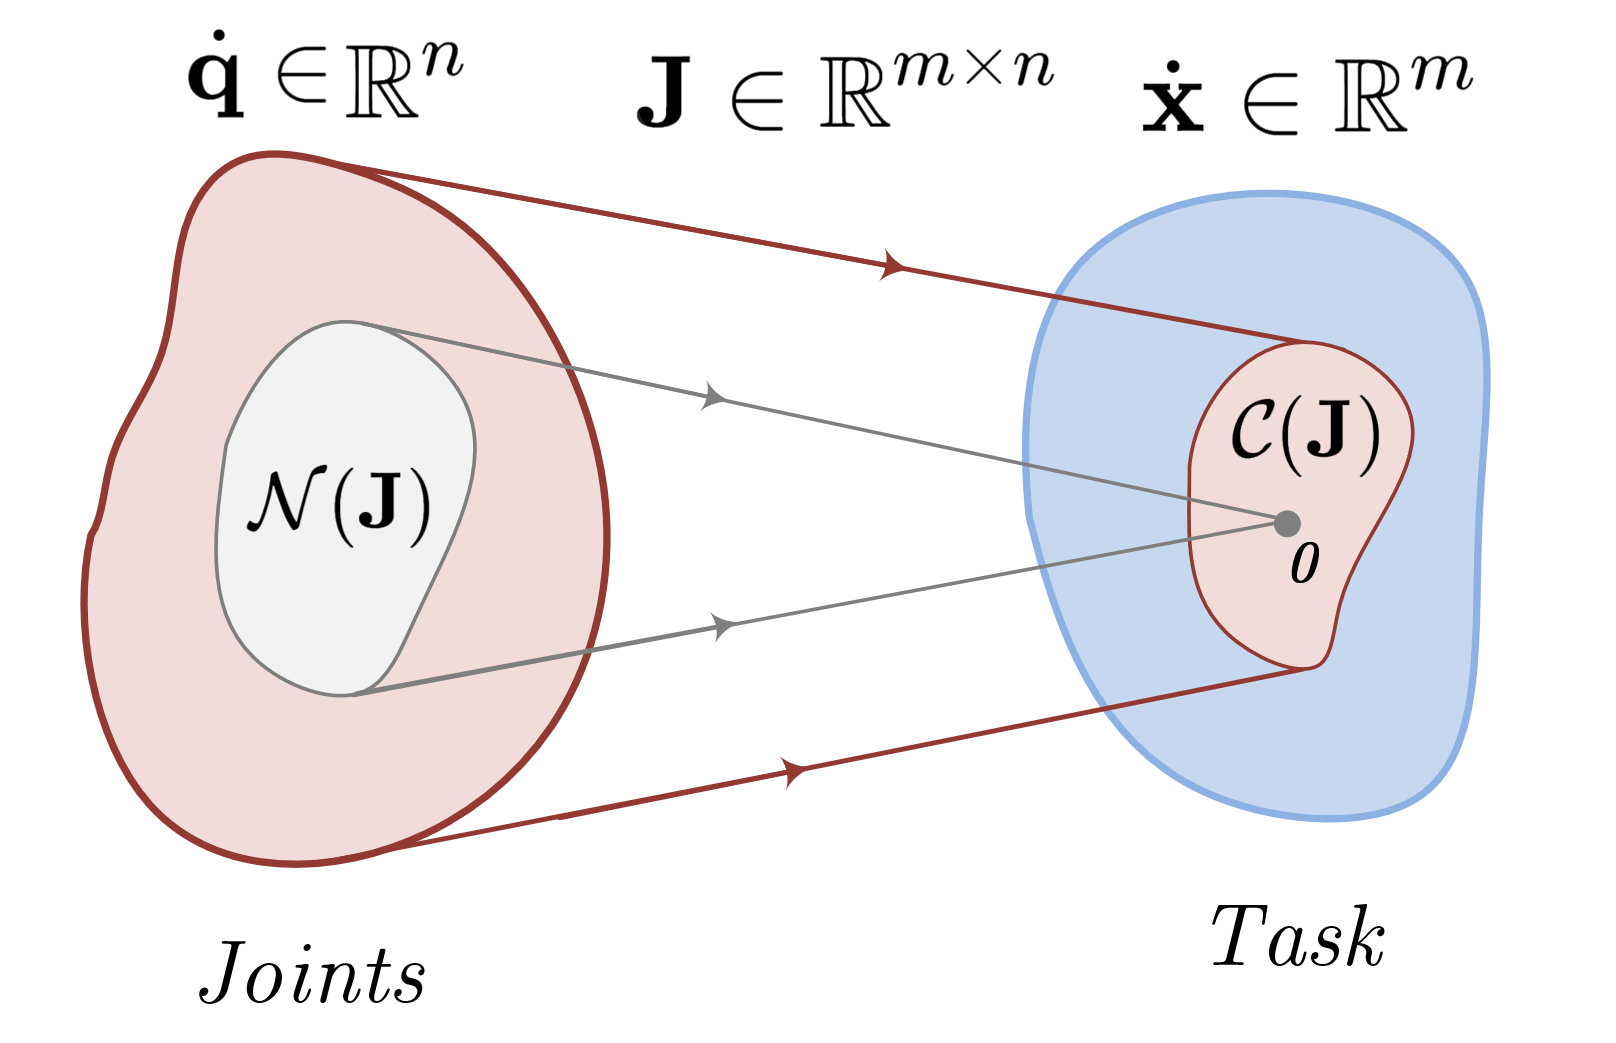
\includegraphics[height=4cm,width=1\textwidth,keepaspectratio]{jacobian_mapping.PNG}}
    \caption{Click for google Collab}
    \label{fig:jacobian_mapping.PNG}
\end{figure}
\end{column}
\begin{column}{0.54\textwidth}
    Let us consider differential kinematic relationship:
    \begin{equation}
        \dot{\boldsymbol{x}} = \mathbf{J}(\mathbf{q})\dot{\mathbf{q}}
    \end{equation}
    where
    \begin{itemize}
        \item   $\boldsymbol{x} \in \mathbb{R}^m$ task space variables (for instance Cartesian coordinates)
        \item   $\mathbf{q} \in \mathbb{R}^n$ joint space variables (positions of joints)
        \item   $\mathbf{J} \in \mathbb{R}^{m\times n}$ manipulator Jacobian
    \end{itemize}
\end{column}
\end{columns}
\end{frame}

\begin{frame}[t]{Null Space: Application from robotics}
    \framesubtitle{Theory (2)}
    \vspace{-0.6cm}
    \begin{figure}[H]
        \centering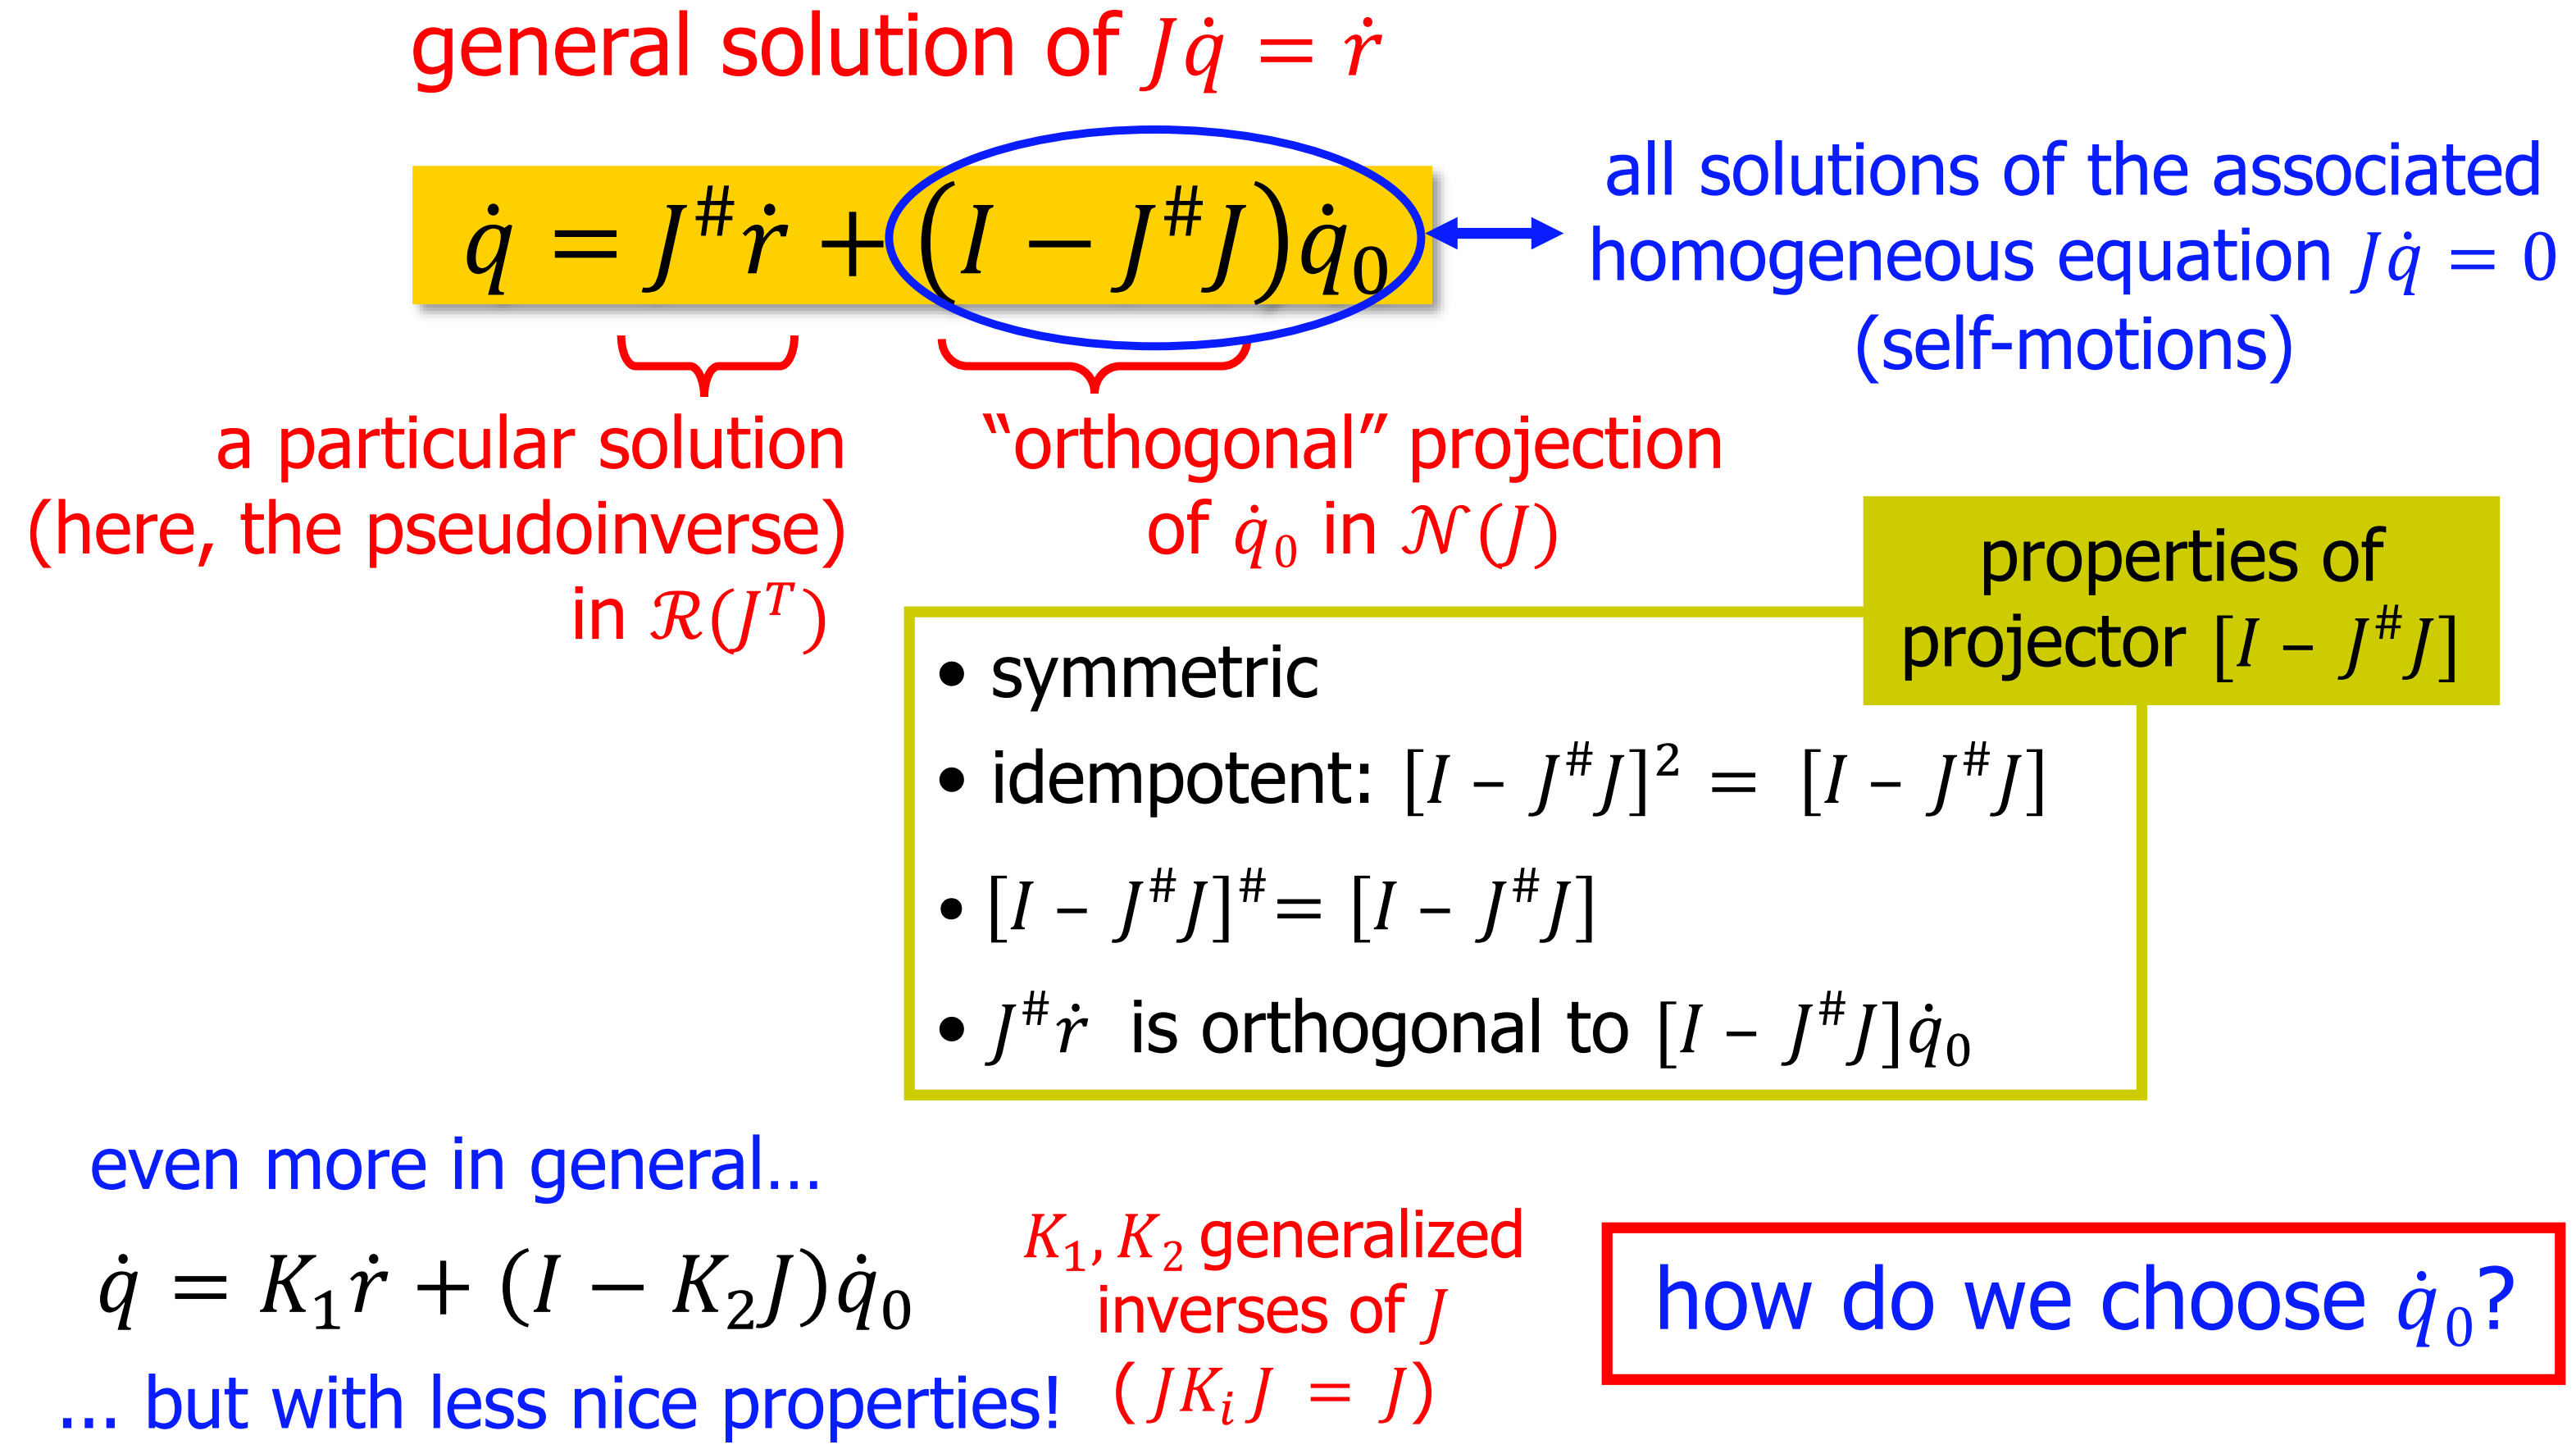
\includegraphics[height=6cm,width=1\textwidth,keepaspectratio]{rob_app_general_idea.png}
        % \caption{caption_name}
        \label{fig:rob_app_general_idea.png}
    \end{figure}
\end{frame}

\begin{frame}[t]{Null Space: Application from robotics}
    \framesubtitle{Theory (3)}
    \vspace{-0.6cm}
    \begin{figure}[H]
        \centering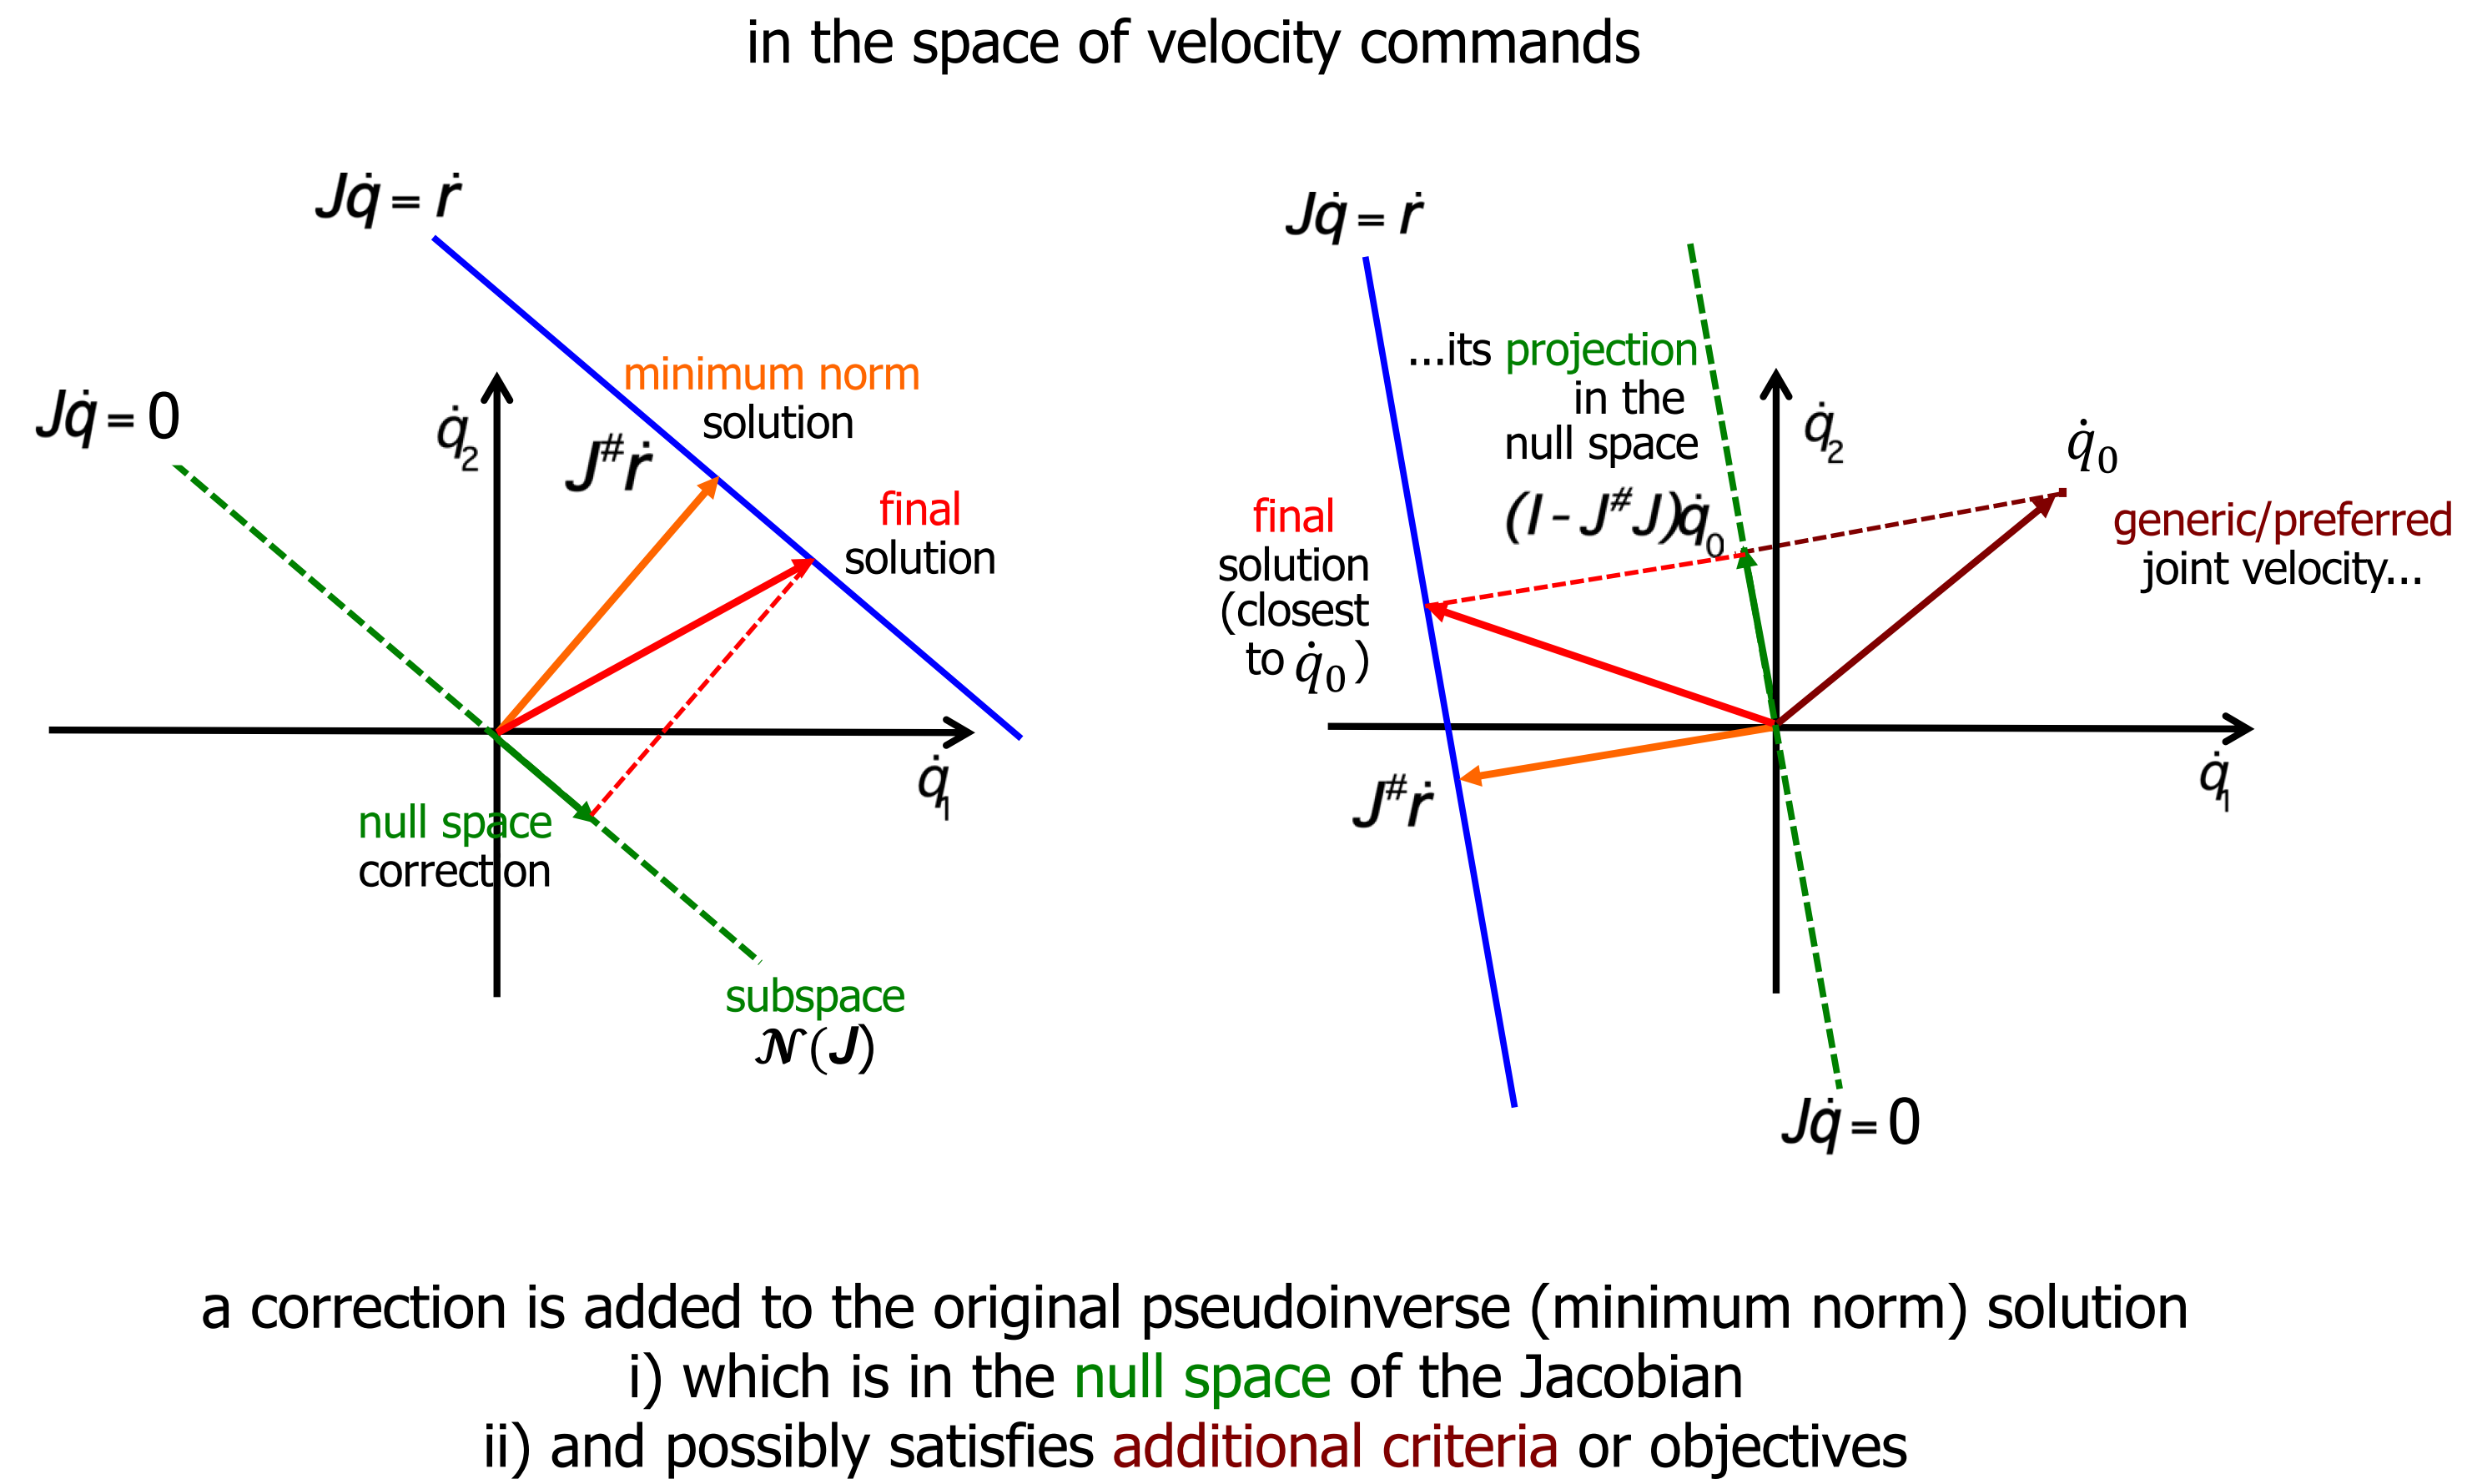
\includegraphics[height=6cm,width=1\textwidth,keepaspectratio]{rob_app_geometry.png}
        % \caption{caption_name}
        \label{fig:rob_app_geometry.png}
    \end{figure}
\end{frame}



\begin{frame}[t]{Task 1}
    \framesubtitle{}
    \begin{figure}[H]
        \centering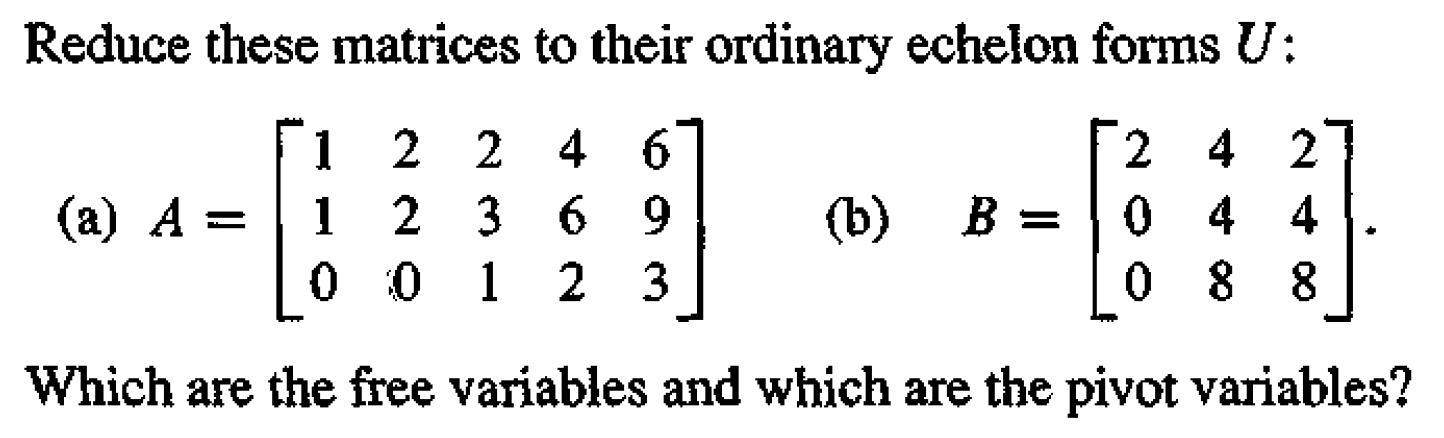
\includegraphics[height=3cm,width=1\textwidth,keepaspectratio]{1.png}
        % \caption{caption_name}
        \label{fig:1.png}
    \end{figure}
    \uncover<2->{
        \alert{\Large Answer}
        \begin{figure}[H]
            \centering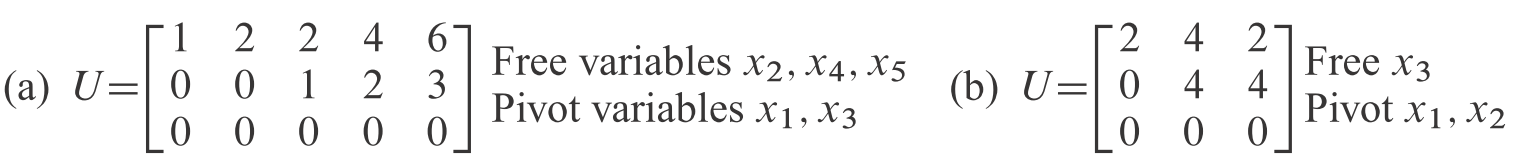
\includegraphics[height=3cm,width=1\textwidth,keepaspectratio]{1ans.png}
            % \caption{caption_name}
            \label{fig:1ans.png}
        \end{figure}
    }
\end{frame}


\note{U --- ref, R --- rref}

\begin{frame}[t]{Task 2}
    \framesubtitle{}
    \begin{figure}[H]
        \centering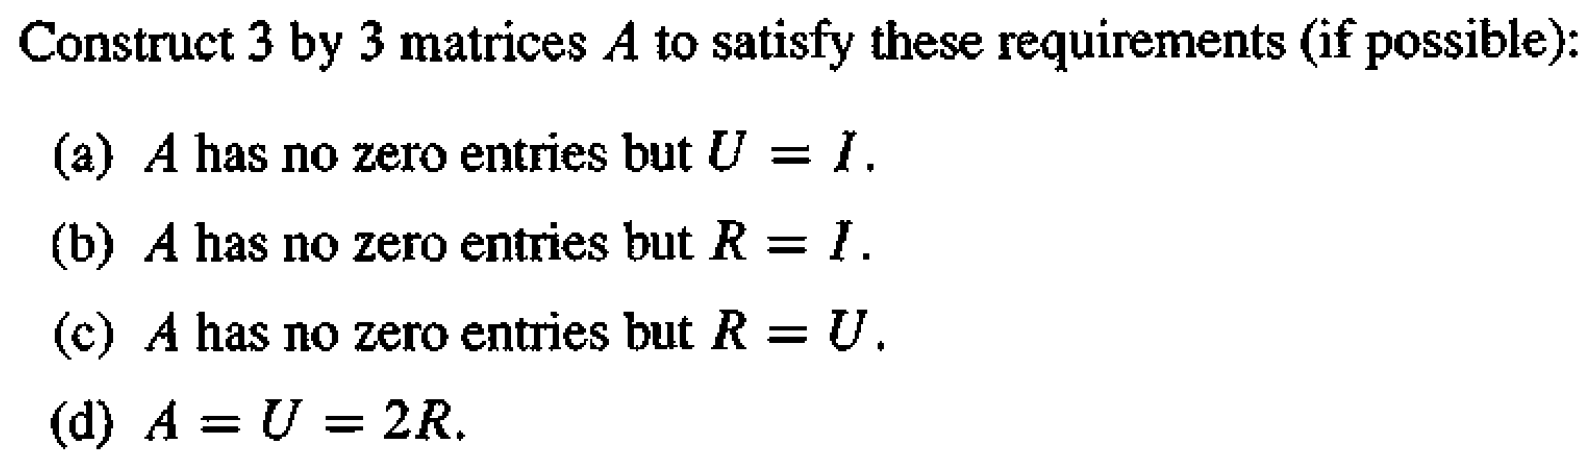
\includegraphics[height=3cm,width=1\textwidth,keepaspectratio]{2.png}
        % \caption{caption_name}
        \label{fig:2.png}
    \end{figure}
    \uncover<2->{
        \alert{\Large Answer}
        \begin{figure}[H]
            \centering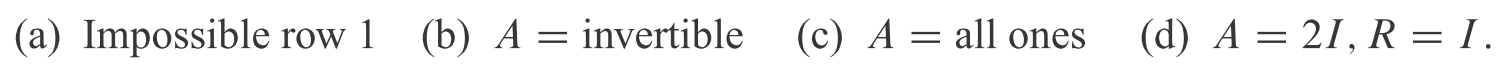
\includegraphics[height=3cm,width=1\textwidth,keepaspectratio]{2ans.png}
            % \caption{caption_name}
            \label{fig:2ans.png}
        \end{figure}
    }
\end{frame}

\begin{frame}[t]{Task 3}
    \framesubtitle{}
    \begin{figure}[H]
        \centering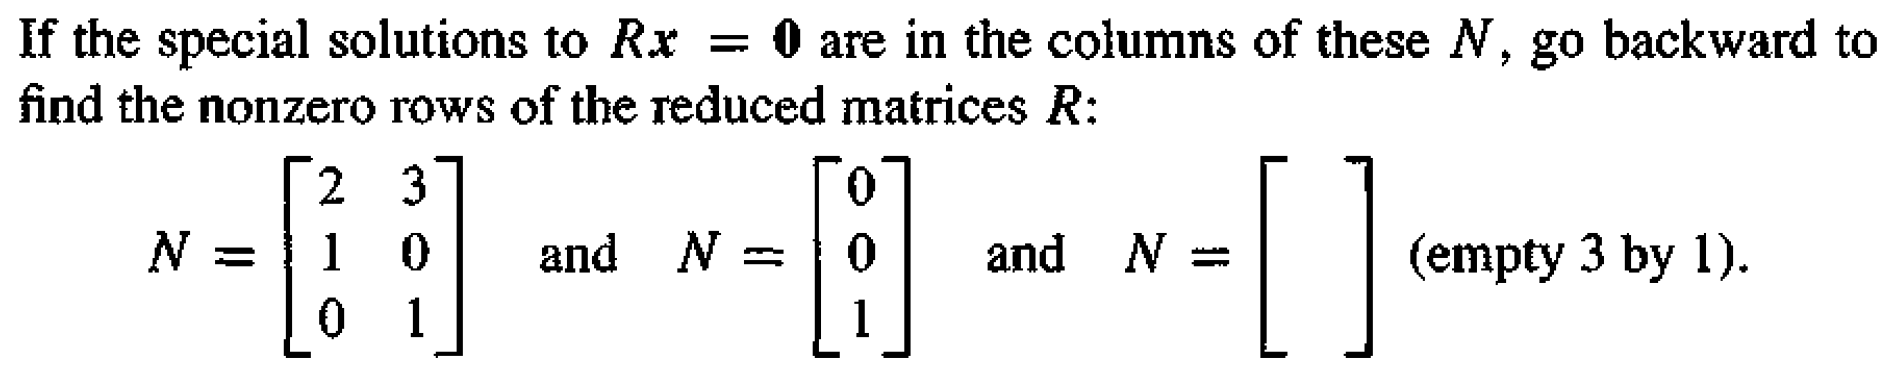
\includegraphics[height=3cm,width=1\textwidth,keepaspectratio]{3.png}
        % \caption{caption_name}
        \label{fig:3.png}
    \end{figure}
    \uncover<2->{
        \alert{\Large Answer}
        \begin{figure}[H]
            \centering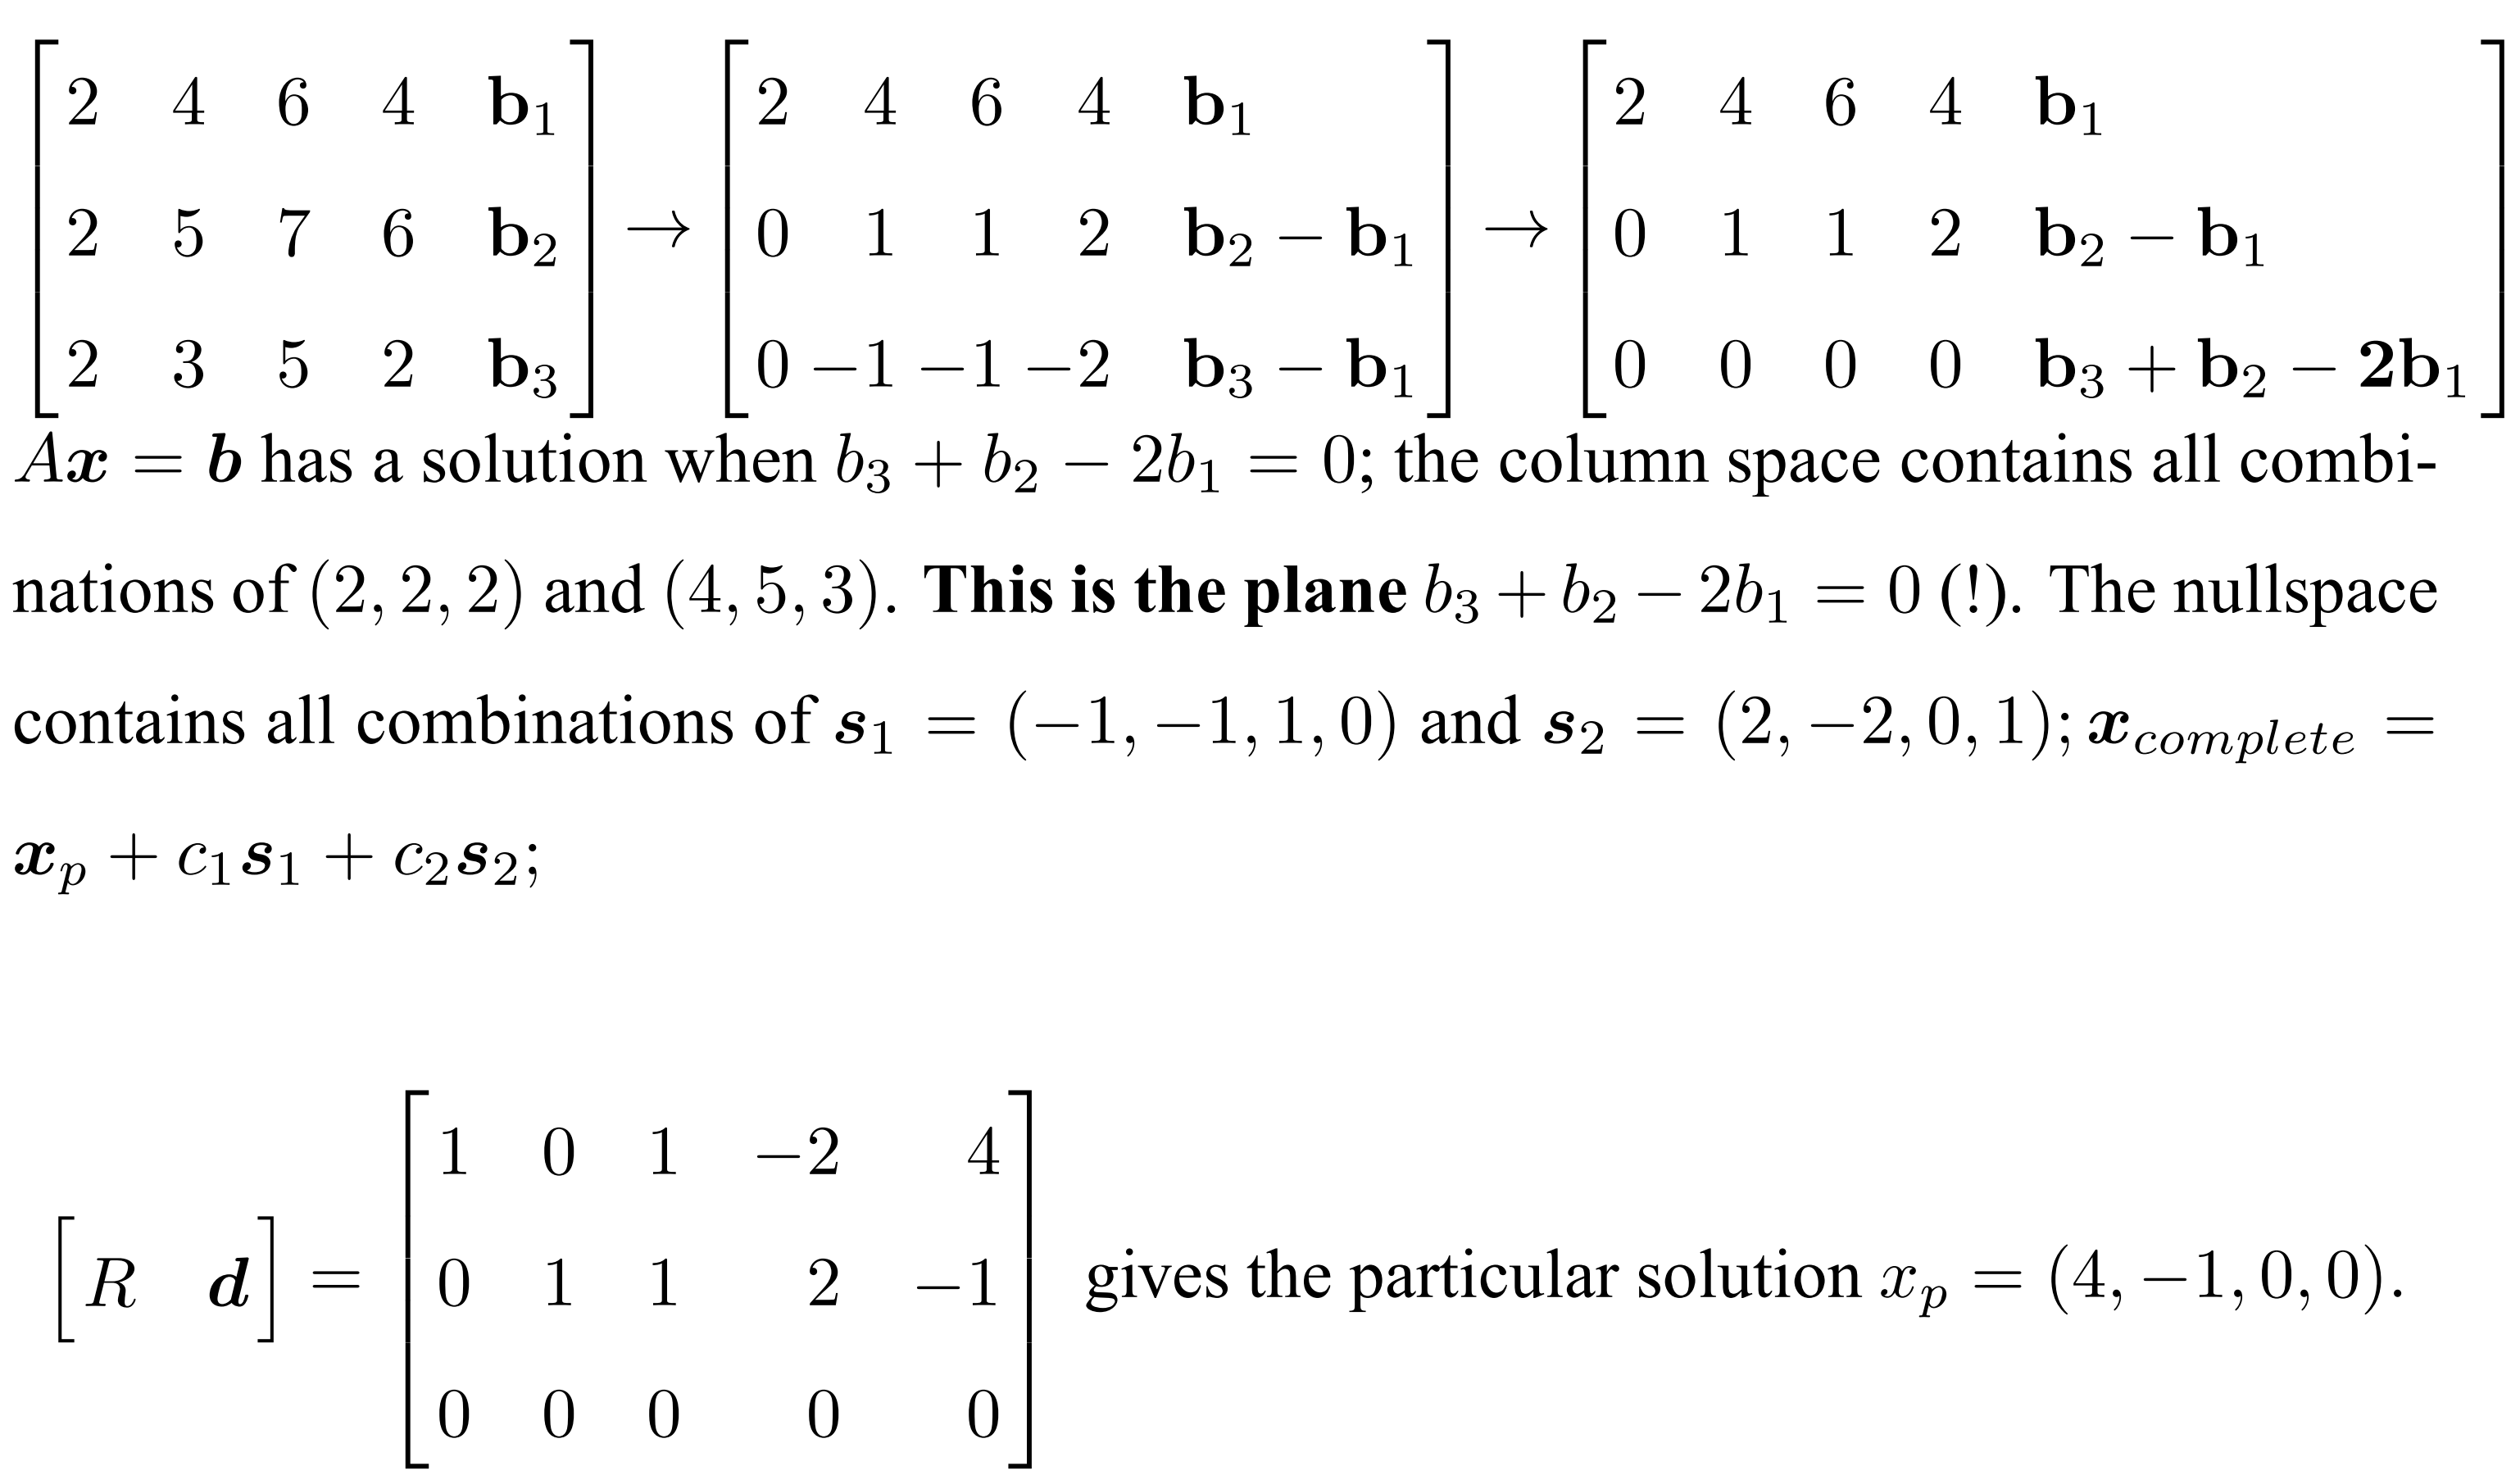
\includegraphics[height=3cm,width=1\textwidth,keepaspectratio]{3ans.png}
            % \caption{caption_name}
            \label{fig:3ans.png}
        \end{figure}
    }
\end{frame}

\begin{frame}[t]{Reference material}
    \framesubtitle{}
    \Large
    \begin{itemize}
        \item \href{http://diag.uniroma1.it/~deluca/rob2_en.php}{Robotics 2 course from Sapienza}
        \item \textit{"Linear Algebra and Applications", pdf pages 87--101 } \\ 2.1-2.2
        \item \textit{"Introduction to Linear Algebra", pdf pages 132--152 }\\  3.1 -- 3.2
        \item \href{https://youtu.be/95KM1JWs_Bg}{this lab video, 2022 year}
    \end{itemize}
\end{frame}

\begin{frame}[t]{Preparation material for the next class}
    \Large
    \begin{itemize}
        \item \href{https://www.youtube.com/watch?v=yjBerM5jWsc&list=PL49CF3715CB9EF31D&index=9}{Lecture 9 and 10}
        \item \textit{"Linear Algebra and Applications", pdf pages 139--149 }\\ The application of four fundamental subspaces in CS
        \item \href{https://youtu.be/yfj8uMwAgrI}{Matrix Transpose and the Four Fundamental Subspaces}\\ Video is about how $A$ transpose appeared
        \item \href{https://matworld.ru/calculator/matrix-calculator-1.php}{Matrix online calculator}(russian)
    \end{itemize}
\end{frame}

\fbckg{fibeamer/figs/last_page.png}
\frame[plain]{}

\end{document}